%==============================================================================
\section{Query Decomposition}
\label{sec:decomposition}
%==============================================================================

This section presents our query decomposition framework, which rewrites multi-hop queries to maximize the use of \onehop operations.

%------------------------------------------------------------------------------
\subsection{Motivation}
\label{sec:decomposition:motivation}
%------------------------------------------------------------------------------

Consider a 3-hop chain query:
\begin{center}
\small
\texttt{(a1:Account)-[t1]$\rightarrow$(a2)-[t2]$\rightarrow$(a3)-[t3]$\rightarrow$(a4)}\\
\texttt{WHERE a1.balance > 10000 AND a4.balance < 1000}
\end{center}

Without decomposition, this becomes a 7-way join processed entirely by the oblivious multi-way join algorithm. With decomposition, we can:
\begin{enumerate}
    \item Apply \onehop to $(a1, t1, a2)$ with the filter on $a1$ $\rightarrow$ produces $H_1$
    \item Apply \onehop to $(a3, t3, a4)$ with the filter on $a4$ $\rightarrow$ produces $H_2$
    \item Reduce the query to: $H_1 \bowtie t2 \bowtie H_2$ (only 3 tables)
\end{enumerate}

The reduced query is faster because: (1) \onehop is more efficient than the equivalent portion of multi-way join, and (2) the remaining join has fewer tables.

% %------------------------------------------------------------------------------
% \subsection{Decomposition Problem}
% \label{sec:decomposition:problem}
% %------------------------------------------------------------------------------

% \paragraph{Input:}
% A query graph $G_Q = (V_Q, E_Q)$ where:
% \begin{itemize}
%     \item $V_Q$ = node table references (possibly with predicates)
%     \item $E_Q$ = edge table references connecting nodes
% \end{itemize}

% \paragraph{Output:}
% \begin{itemize}
%     \item A set of \onehop operations $\{H_1, \ldots, H_k\}$
%     \item A reduced query $Q'$ over the \onehop outputs and remaining tables
% \end{itemize}

% \paragraph{Goal:}
% Minimize total execution cost while maintaining correctness and security.

% %------------------------------------------------------------------------------
% \subsection{Decomposition Algorithm}
% \label{sec:decomposition:algorithm}
% %------------------------------------------------------------------------------

% Algorithm~\ref{alg:decompose} shows our greedy decomposition procedure.

% \begin{algorithm}[t]
% \caption{Query Decomposition}
% \label{alg:decompose}
% \begin{algorithmic}[1]
% \Require Query graph $G_Q = (V_Q, E_Q)$
% \Ensure Set of \onehop operations, reduced query $Q'$

% \State $\mathcal{H} \leftarrow \emptyset$ \Comment{Set of 1-hop operations}
% \State $\mathcal{T} \leftarrow$ identify all $(node, edge, node)$ triplets in $G_Q$

% \For{each triplet $T = (n_1, e, n_2) \in \mathcal{T}$}
%     \State $score(T) \leftarrow$ compute optimization potential
% \EndFor

% \State Sort $\mathcal{T}$ by score (descending)

% \For{each triplet $T = (n_1, e, n_2)$ in sorted order}
%     \If{$T$ does not overlap with any triplet in $\mathcal{H}$}
%         \State $\mathcal{H} \leftarrow \mathcal{H} \cup \{T\}$
%         \State Execute $H_T \leftarrow$ \onehop$(n_1, e, n_2)$
%     \EndIf
% \EndFor

% \State Construct $Q'$ by replacing each $T \in \mathcal{H}$ with $H_T$
% \STATE \RETURN $\mathcal{H}$, $Q'$
% \end{algorithmic}
% \end{algorithm}

% \paragraph{Scoring Triplets.}
% We score each triplet based on its optimization potential:
% \begin{itemize}
%     \item \textbf{Has filter predicates}: Triplets containing filtered nodes score higher, as \onehop can apply filters efficiently.
%     \item \textbf{Reduces join width}: Triplets that replace more tables in the join score higher.
%     \item \textbf{Edge table size}: Larger edge tables benefit more from \onehop's efficiency.
% \end{itemize}

% \paragraph{Non-Overlapping Selection.}
% Two triplets \emph{overlap} if they share an edge table. We select triplets greedily, skipping any that overlap with already-selected ones. This ensures each edge table is processed at most once.

%------------------------------------------------------------------------------
\subsection{Example: Chain Query Decomposition}
\label{sec:decomposition:example}
%------------------------------------------------------------------------------

\begin{figure}[t]
\centering
\small
\begin{verbatim}
Original Query (3-hop chain):
  (a1)--[t1]-->(a2)--[t2]-->(a3)--[t3]-->(a4)

Triplets identified:
  T1 = (a1, t1, a2)  
  T2 = (a2, t2, a3)  
  T3 = (a3, t3, a4) 

Selected (non-overlapping): T1, T3

After decomposition:
  H1 = ForwardFill(a1, t1, a2)  [size = |t1|]
  H2 = ForwardFill(a3, t3, a4)  [size = |t3|]
  Q' = H1 --[t2]--> H2          [3-way join]
\end{verbatim}
\caption{Decomposition of a 3-hop chain query. The 7-table join becomes two \onehop operations plus a 3-table join.}
\label{fig:decomposition}
\end{figure}

Figure~\ref{fig:decomposition} illustrates the decomposition of a 3-hop chain query. The original 7-table join is reduced to two \onehop operations (executed independently) plus a 3-table multi-way join.

%------------------------------------------------------------------------------
\subsection{Correctness and Optimality}
\label{sec:decomposition:correctness}
%------------------------------------------------------------------------------

\paragraph{Correctness.}
The decomposition is correct because \onehop computes exactly the same result as the corresponding three-way join. Replacing a triplet $(n_1, e, n_2)$ with $H = \onehop(n_1, e, n_2)$ produces semantically equivalent results.

\paragraph{Optimality.}
Finding the optimal decomposition is NP-hard in general (reducible from maximum independent set on the triplet overlap graph). Our greedy algorithm provides a 2-approximation for chain queries and works well in practice for common query patterns.


%==============================================================================
\section{Security Analysis}
\label{sec:security}
%==============================================================================

This section provides an informal security argument for the complete \system pipeline.

%------------------------------------------------------------------------------
\subsection{Security Claim}
\label{sec:security:claim}
%------------------------------------------------------------------------------

\begin{theorem}[Security]
The complete \system pipeline (decomposition + \onehop + multi-way join) leaks only information that is public by our threat model:
\begin{enumerate}
    \item Base table sizes ($|S|$, $|E|$, $|D|$, etc.)
    \item Query structure (which tables are joined, predicates)
    \item Final output size
\end{enumerate}
\end{theorem}

%------------------------------------------------------------------------------
\subsection{Argument}
\label{sec:security:argument}
%------------------------------------------------------------------------------

\paragraph{\onehop Security.}
As shown in Section~\ref{sec:onehop:security}, each \onehop operation is oblivious. The output size equals the edge table size, which is public. Key properties:
\begin{itemize}
    \item Duplicate suppression hides node degrees
    \item Forward fill has data-independent access patterns
    \item Output padding hides predicate selectivity
\end{itemize}

\paragraph{Composition Security.}
The outputs of \onehop operations become inputs to the oblivious multi-way join. Because:
\begin{enumerate}
    \item Each \onehop output has a publicly known size (= edge table size)
    \item The multi-way join algorithm~\cite{ruidi2025oblivious} is proven secure when input sizes are public
\end{enumerate}
The composition remains secure. The multi-way join sees inputs of known sizes and produces output while hiding intermediate results.

\paragraph{Decomposition Security.}
Query decomposition is a compile-time transformation based on query structure (public). It does not depend on data values. The choice of which triplets to optimize is deterministic given the query, revealing nothing about the data.

%------------------------------------------------------------------------------
\subsection{What Is Not Leaked}
\label{sec:security:notleaked}
%------------------------------------------------------------------------------

The following remain hidden from the adversary:
\begin{itemize}
    \item \textbf{Data values}: Actual node/edge properties
    \item \textbf{Predicate selectivity}: What fraction of rows satisfy filters
    \item \textbf{Node degrees}: How many edges each node has
    \item \textbf{Join selectivity}: How many tuples actually match
    \item \textbf{Intermediate cardinalities}: Sizes of partial results during multi-way join
\end{itemize}


%==============================================================================
\section{Evaluation}
\label{sec:evaluation}
%==============================================================================

We evaluate \system on financial transaction workloads, comparing decomposed execution against baseline oblivious multi-way joins.

%------------------------------------------------------------------------------
\subsection{Experimental Setup}
\label{sec:evaluation:setup}
%------------------------------------------------------------------------------

\paragraph{Hardware.}
Intel Xeon processor with TDX support, 128GB RAM, running Ubuntu 22.04.

\paragraph{Dataset.}
Banking transaction graph with:
\begin{itemize}
    \item \texttt{Account} nodes: varying from 1K to 100K
    \item \texttt{Transaction} edges: 5$\times$ the number of accounts
    \item Properties: account balance, transaction amount, timestamps
\end{itemize}

\paragraph{Queries.}
\begin{itemize}
    \item \textbf{Chain queries}: 2-hop to 5-hop linear patterns
    \item \textbf{Branch queries}: Star patterns with central node
    \item All queries include filter predicates on endpoint nodes
\end{itemize}

\paragraph{Baselines.}
\begin{itemize}
    \item \textbf{No Decomposition}: All tables processed by oblivious multi-way join
    \item \textbf{With Decomposition}: \system's hybrid approach
\end{itemize}

%------------------------------------------------------------------------------
\subsection{End-to-End Performance}
\label{sec:evaluation:e2e}
%------------------------------------------------------------------------------

Table~\ref{tab:e2e} shows end-to-end query execution times.

\begin{table}[t]
\centering
\caption{End-to-end performance comparison (10K accounts, 50K transactions)}
\label{tab:e2e}
\begin{tabular}{lrrr}
\toprule
\textbf{Query} & \textbf{No Decomp} & \textbf{With Decomp} & \textbf{Speedup} \\
\midrule
4-hop chain & 11.53s & 6.94s & 1.66$\times$ \\
branch & 23.03s & 16.97s & 1.35$\times$ \\
\bottomrule
\end{tabular}
\end{table}

\paragraph{Key Findings.}
\begin{itemize}
    \item \system achieves 1.35--1.66$\times$ speedup on these queries
    \item Chain queries benefit more than branch queries from decomposition
    \item The one-hop operator contributes only 0.17s of the 6.94s decomposed time (2.5\%), with most time in the reduced multi-way join
\end{itemize}

% %------------------------------------------------------------------------------
% \subsection{Breakdown Analysis}
% \label{sec:evaluation:breakdown}
% %------------------------------------------------------------------------------

% Figure~\ref{fig:breakdown} shows the time breakdown for a 4-hop chain query.

% \begin{figure}[t]
% \centering
% \small
% \begin{verbatim}
% 4-hop chain query breakdown (10K accounts):

% No Decomposition:
%   [======= Multi-way Join: 11.53s =======]

% With Decomposition:
%   [1-hop][======= Reduced MWJ =======]
%    0.17s          6.77s
%               Total: 6.94s
% \end{verbatim}
% \caption{Time breakdown for 4-hop chain query. The \onehop operation is extremely fast (0.17s), while the main benefit comes from the reduced multi-way join operating on fewer tables.}
% \label{fig:breakdown}
% \end{figure}

% The \onehop operation (0.17s) is nearly negligible compared to the join time. The key benefit is that the reduced multi-way join (6.77s) operates on the decomposed query structure, which is faster than the original 7-table join (11.53s).

%------------------------------------------------------------------------------
\subsection{Scaling Experiments}
\label{sec:evaluation:scaling}
%------------------------------------------------------------------------------

\paragraph{Scaling with Data Size.}
Table~\ref{tab:scaling} shows performance as data size increases.

\begin{table}[t]
\centering
\caption{Scaling with data size (4-hop chain query)}
\label{tab:scaling}
\begin{tabular}{rrrr}
\toprule
\textbf{Accounts} & \textbf{No Decomp} & \textbf{With Decomp} & \textbf{Speedup} \\
\midrule
1K & 0.68s & 0.40s & 1.67$\times$ \\
2K & 1.39s & 0.74s & 1.86$\times$ \\
5K & 4.09s & 3.50s & 1.16$\times$ \\
10K & 11.53s & 6.94s & 1.66$\times$ \\
20K & 22.01s & 14.62s & 1.50$\times$ \\
50K & 70.00s & 36.87s & 1.89$\times$ \\
\bottomrule
\end{tabular}
\end{table}

Speedup ranges from 1.16$\times$ to 1.89$\times$ across different scales, with an average of approximately 1.6$\times$. The variation is due to cache effects and the relative cost of different phases at different scales.

\paragraph{One-Hop Overhead.}
The one-hop operator time scales linearly with data size: 0.01s at 1K accounts to 1.01s at 50K accounts, representing only 1--3\% of total decomposed execution time.

Figure~\ref{fig:scaling} visualizes the scaling behavior for both query types. The decomposed approach (blue) consistently outperforms the non-decomposed baseline (red), with speedup annotations showing the improvement ratio at each scale.

\begin{figure*}[t]
\centering
\begin{minipage}[t]{0.48\textwidth}
    \centering
    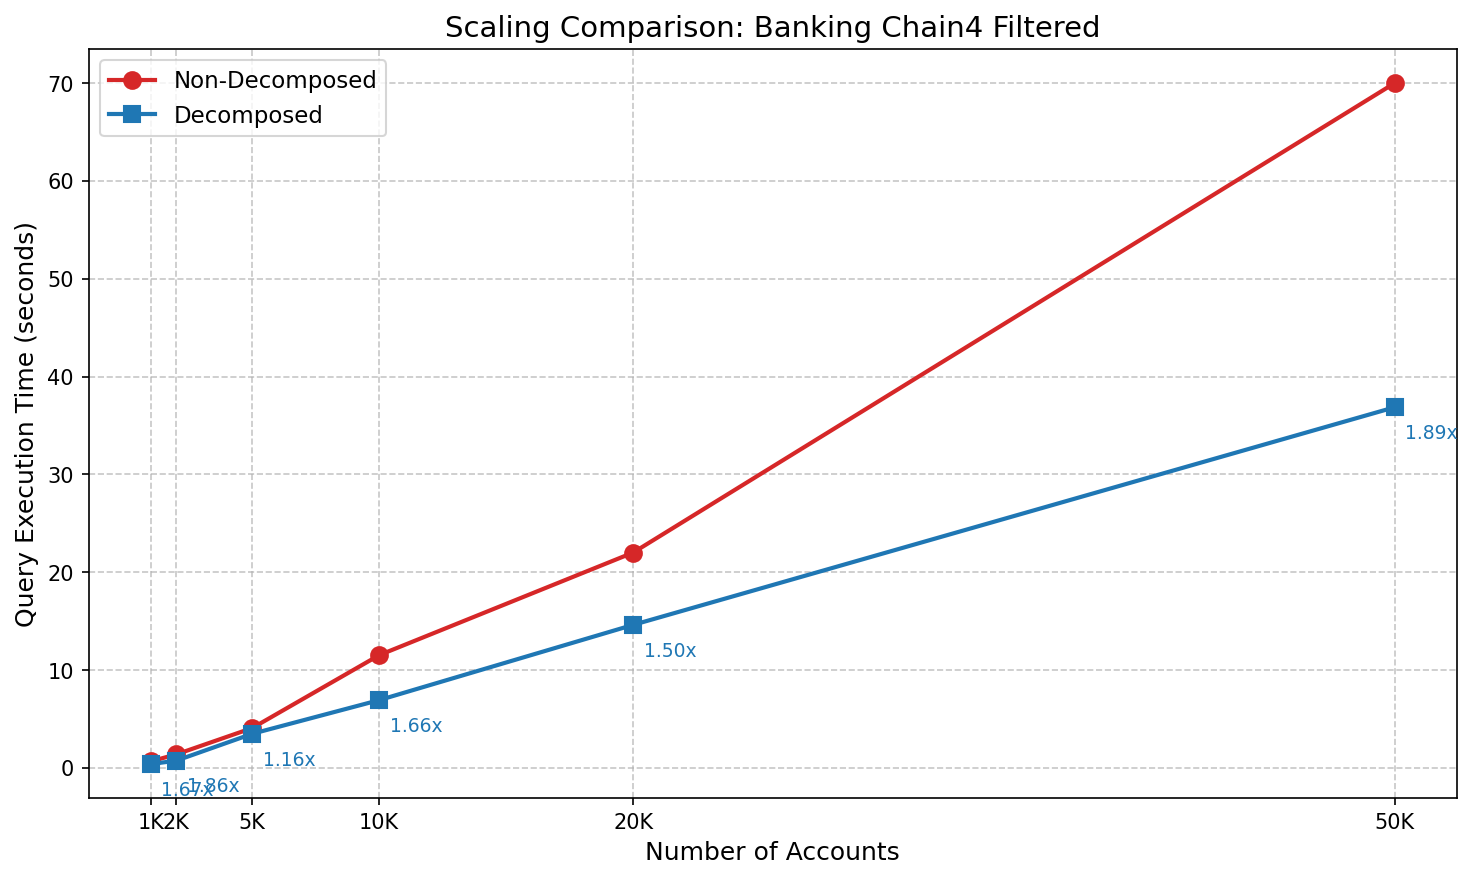
\includegraphics[width=\textwidth]{figures/scaling_chain4.png}
    (a) 4-hop chain query
\end{minipage}
\hfill
\begin{minipage}[t]{0.48\textwidth}
    \centering
    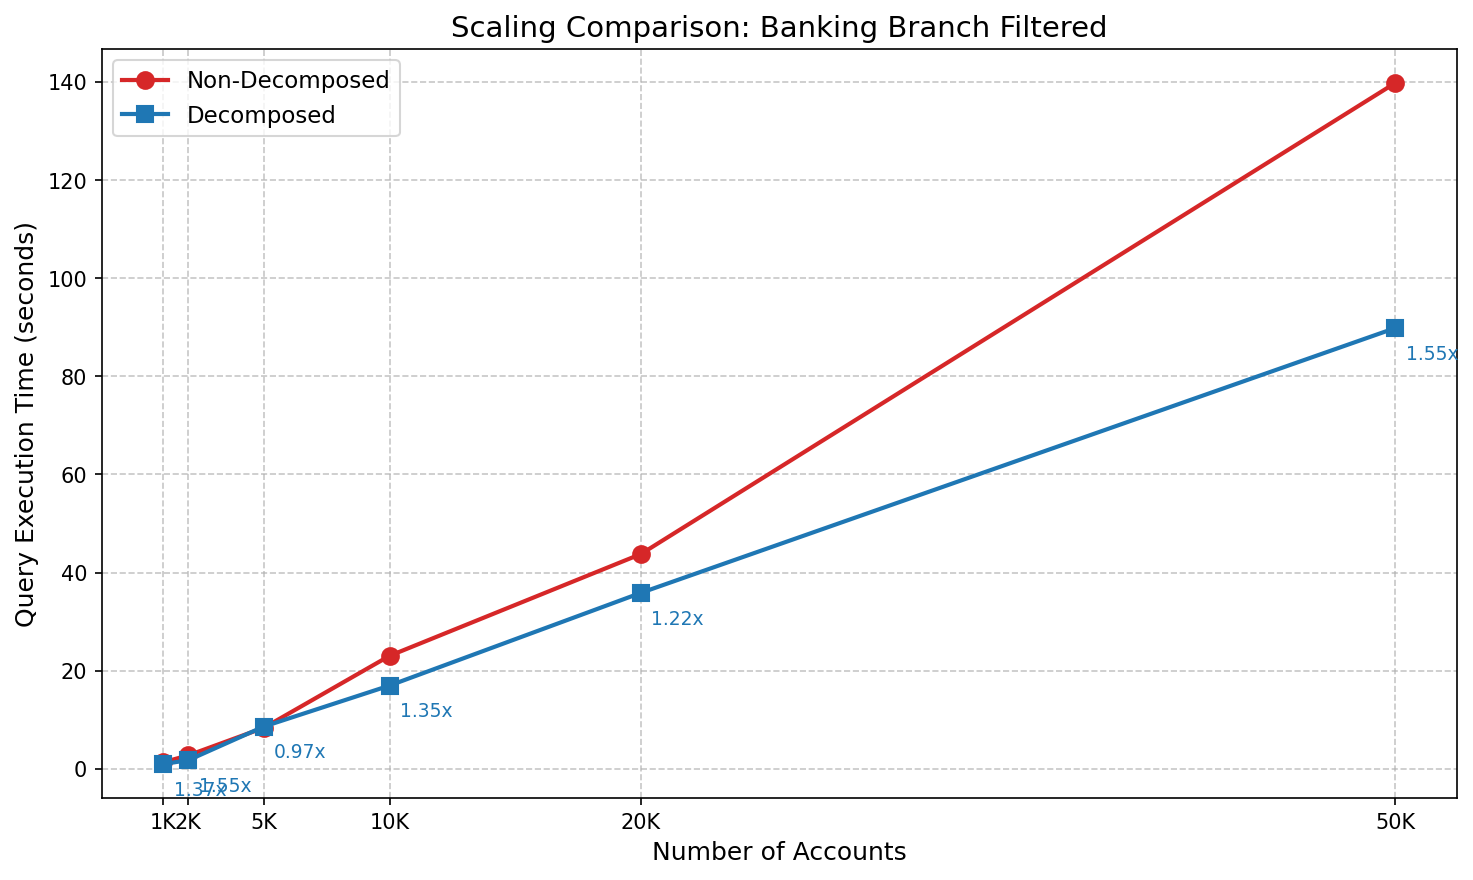
\includegraphics[width=\textwidth]{figures/scaling_branch.png}
    (b) Branch query
\end{minipage}
\caption{Scaling performance: Non-decomposed (red) vs decomposed (blue) execution time as data size increases. Speedup annotations show the ratio at each scale.}
\label{fig:scaling}
\end{figure*}



% %==============================================================================
% \section{Related Work}
% \label{sec:related}
% %==============================================================================

% %------------------------------------------------------------------------------
% \subsection{Oblivious Database Systems}
% \label{sec:related:oblivious}
% %------------------------------------------------------------------------------

% \paragraph{ORAM-Based Approaches.}
% Oblivious RAM~\cite{oram-goldreich} provides general-purpose oblivious memory access but incurs $O(\log N)$ overhead per access. Systems like Oblix~\cite{oblix} and Opaque~\cite{opaque} use ORAM for oblivious database operations. Our work avoids ORAM overhead by designing algorithms with inherently oblivious access patterns.

% \paragraph{Oblivious Relational Operators.}
% Prior work has developed oblivious versions of relational operators: sorting~\cite{oblivious-sort}, filtering, aggregation, and joins~\cite{oblivious-join}. We build on oblivious multi-way join algorithms~\cite{TODO} but introduce graph-specific optimizations.

% %------------------------------------------------------------------------------
% \subsection{Secure Graph Processing}
% \label{sec:related:graph}
% %------------------------------------------------------------------------------

% \paragraph{Encrypted Graph Databases.}
% Systems like encrypted Neo4j variants protect data at rest but do not hide access patterns during query execution.

% \paragraph{TEE-Based Graph Analytics.}
% GraphSC~\cite{graphsc} and similar systems run graph analytics (PageRank, shortest paths) inside secure enclaves. These focus on iterative algorithms, not pattern-matching queries. Our work targets the latter.

% \paragraph{Oblivious Graph Algorithms.}
% Prior work on oblivious graph algorithms focuses on specific computations (BFS, DFS, shortest paths). We address the more general problem of pattern-matching queries with predicates.

% %------------------------------------------------------------------------------
% \subsection{Graph Query Optimization}
% \label{sec:related:optimization}
% %------------------------------------------------------------------------------

% Traditional graph query optimization focuses on join ordering, indexing, and caching---none of which consider obliviousness. Query decomposition appears in distributed graph processing but without security constraints. To our knowledge, \system is the first to combine graph-native query optimization with oblivious execution.


%==============================================================================
\section{Conclusion}
\label{sec:conclusion}
%==============================================================================

We presented \system, an oblivious property graph database that exploits graph structure for efficient secure query processing. Our key contributions are:

\begin{enumerate}
    \item \textbf{\onehop}: An oblivious one-hop operator that uses duplicate suppression and forward filling to achieve data-independent access patterns. By producing output of publicly known size (= edge table size), \onehop enables graph-native optimization without information leakage.

    \item \textbf{Query Decomposition}: A framework that rewrites multi-hop queries to maximize \onehop usage, reducing the work for oblivious multi-way joins.

    \item \textbf{Evaluation}: Experiments on financial transaction workloads showing 1.2--1.9$\times$ speedup over baseline oblivious execution while maintaining identical security guarantees.
\end{enumerate}

\system demonstrates that graph-specific optimizations are compatible with oblivious execution. Future work includes extending to cyclic query patterns, developing cost-based decomposition, and supporting additional graph operations.

